\documentclass[tikz,border=10pt]{standalone}
% Shared style for all project diagrams
\usepackage{amsmath,amssymb}
\usetikzlibrary{positioning,arrows.meta,calc,fit,decorations.pathreplacing}
\renewcommand{\familydefault}{\sfdefault}
\definecolor{accent}{RGB}{42,120,214}
\definecolor{lblue}{RGB}{234,242,252}
\definecolor{card}{RGB}{247,247,245}
\definecolor{ink}{RGB}{17,17,17}
\definecolor{gray52}{RGB}{82,81,78}
\definecolor{dblue}{RGB}{13,54,107}
\tikzset{
  box/.style={draw=accent, thick, rounded corners=3pt, fill=lblue, align=center,
              minimum height=1.05cm, inner sep=6pt, text=ink},
  plain/.style={draw=gray52!60, thick, rounded corners=3pt, fill=card, align=center,
              minimum height=1.05cm, inner sep=6pt, text=ink},
  ghost/.style={align=center, text=gray52, font=\footnotesize},
  arr/.style={-{Stealth[length=2.6mm]}, very thick, draw=accent},
  garr/.style={-{Stealth[length=2.6mm]}, thick, draw=gray52},
  lbl/.style={font=\footnotesize, text=gray52, align=center},
}

\begin{document}
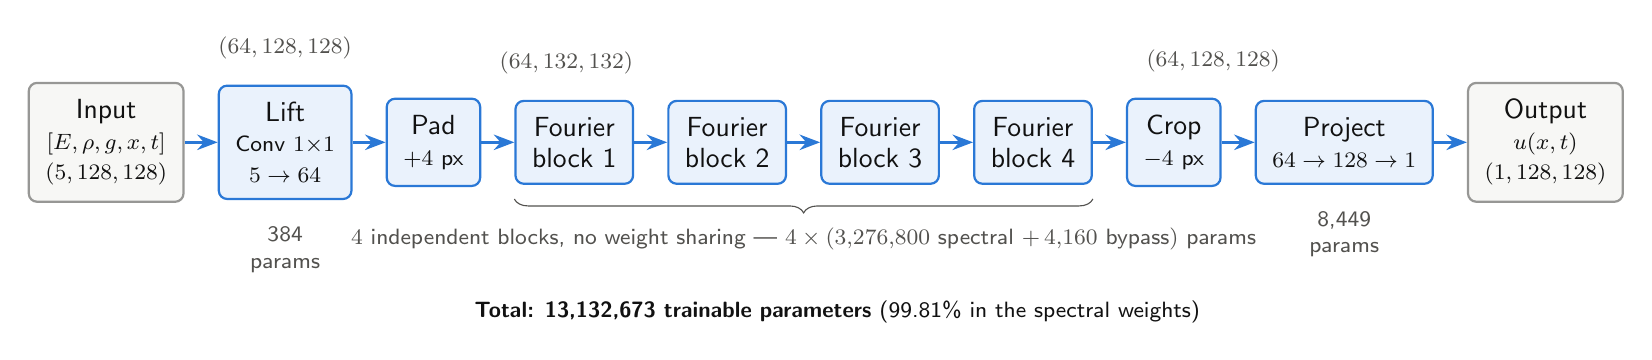
\begin{tikzpicture}[node distance=0.5cm and 0.42cm]
  \node[plain] (inp) {Input\\[-1pt] {\footnotesize $[E,\rho,g,x,t]$}\\[-1pt] {\footnotesize $(5,128,128)$}};
  \node[box, right=of inp]  (lift) {Lift\\[-1pt] {\footnotesize Conv $1{\times}1$}\\[-1pt] {\footnotesize $5\to 64$}};
  \node[box, right=of lift] (pad)  {Pad\\[-1pt] {\footnotesize $+4$ px}};
  \node[box, right=of pad]  (fb1)  {Fourier\\[-1pt] block 1};
  \node[box, right=of fb1]  (fb2)  {Fourier\\[-1pt] block 2};
  \node[box, right=of fb2]  (fb3)  {Fourier\\[-1pt] block 3};
  \node[box, right=of fb3]  (fb4)  {Fourier\\[-1pt] block 4};
  \node[box, right=of fb4]  (crop) {Crop\\[-1pt] {\footnotesize $-4$ px}};
  \node[box, right=of crop] (proj) {Project\\[-1pt] {\footnotesize $64\to128\to1$}};
  \node[plain, right=of proj] (out) {Output\\[-1pt] {\footnotesize $u(x,t)$}\\[-1pt] {\footnotesize $(1,128,128)$}};

  \draw[arr] (inp) -- (lift);
  \draw[arr] (lift) -- (pad);
  \draw[arr] (pad) -- (fb1);
  \draw[arr] (fb1) -- (fb2);
  \draw[arr] (fb2) -- (fb3);
  \draw[arr] (fb3) -- (fb4);
  \draw[arr] (fb4) -- (crop);
  \draw[arr] (crop) -- (proj);
  \draw[arr] (proj) -- (out);

  % parameter annotations
  \node[lbl, below=0.22cm of lift] {384\\ params};
  \node[lbl, below=0.22cm of proj] {8{,}449\\ params};

  \draw[decorate,decoration={brace,mirror,amplitude=5pt},gray52]
    ($(fb1.south west)+(0,-0.18)$) -- ($(fb4.south east)+(0,-0.18)$)
    node[midway, below=7pt, lbl]
    {$4$ independent blocks, no weight sharing --- $4\times(3{,}276{,}800$ spectral $+\,4{,}160$ bypass$)$ params};

  \node[lbl, below=1.35cm of fb2, xshift=1.4cm, text=ink]
    {\textbf{Total: 13{,}132{,}673 trainable parameters} {\footnotesize (99.81\% in the spectral weights)}};

  % padded shape note
  \node[lbl, above=0.20cm of fb1, xshift=-0.1cm] {$(64,132,132)$};
  \node[lbl, above=0.20cm of lift] {$(64,128,128)$};
  \node[lbl, above=0.20cm of crop, xshift=0.5cm] {$(64,128,128)$};
\end{tikzpicture}
\end{document}
